\section{Welding}

	
	As we can see in figure \ref{fig:weldtypes}, welded joints can be classified as \textbf{full penetration} (or \textbf{butt}) or \textbf{fillet} joints.
	
	\begin{SCfigure}[1][bht]
		\centering 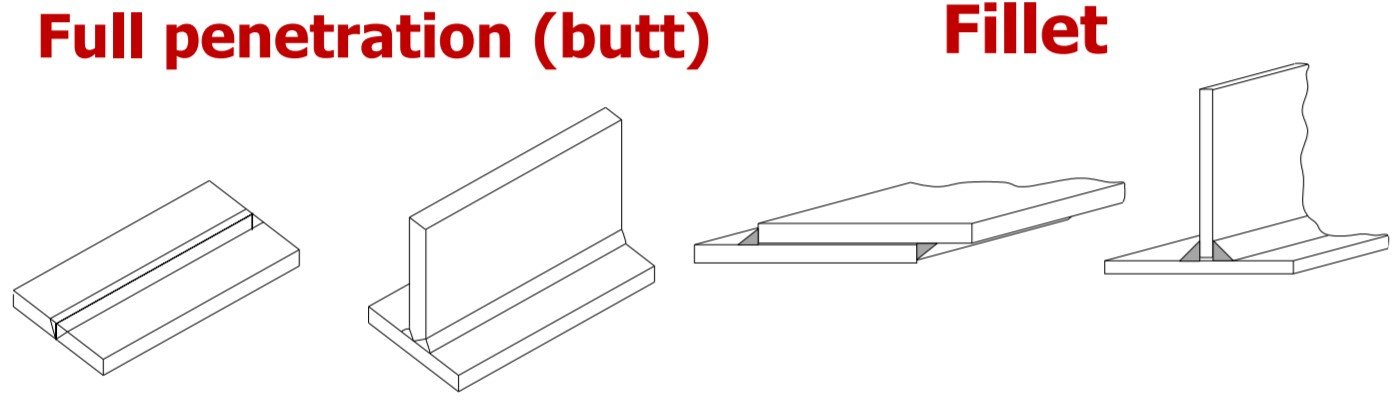
\includegraphics[width=7cm]{weldtypes}
		\caption{classification of welded joints: full penetration (butt) and fillet.} \label{fig:weldtypes}
	\end{SCfigure}

	For such type of welds it's necessary to define the nominal thickness $a$ (of the butt joint of the throat area of the fillet joint), the nominal length $l$ of the joint, the pitch $p$ between the filler blocks (figure \ref{fig:weldsspecs}).
	
	\begin{SCfigure}[1][bht]
		\centering 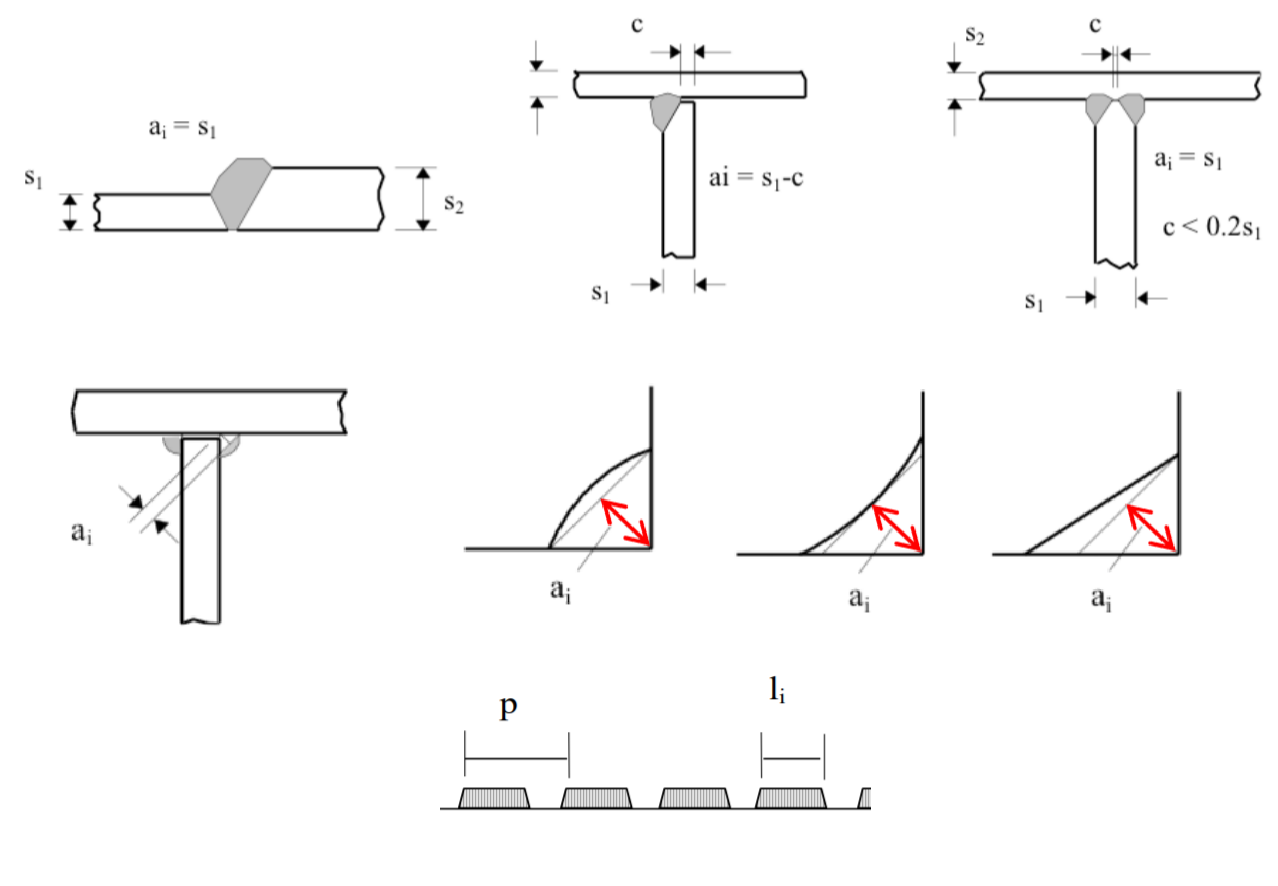
\includegraphics[width=9cm]{weldinggeometry}
		\caption{examples of nominal thickness $a$ for different types of weldings; representation of length $l$ of the joint and the related pitch. } \label{fig:weldsspecs}
	\end{SCfigure}

\subsection{Full penetration joints}
	
	We refer to full penetration joints if the weld is well fabricated and the jointed parts constitute a single structural component without internal discontinuities. With that said also the stress state should be somewhat continuous and we can assume that the weld bead is subjected to a fairly plane stress state with components (that can be seen in figure \ref{fig:fpjstresses}):
	\begin{itemize}
		\item $\sigma_\perp$: normal stress acting along the direction perpendicular to the throat area;
		\item $\sigma_\parallel$: normal stress acting along the direction parallel to the weld bead axis and referred to the cross-section normal to this axis.
		\item $\tau$: shear stresses acting along the direction parallel to the throat area.
	\end{itemize}
	
	\begin{SCfigure}[1][bht]
		\centering 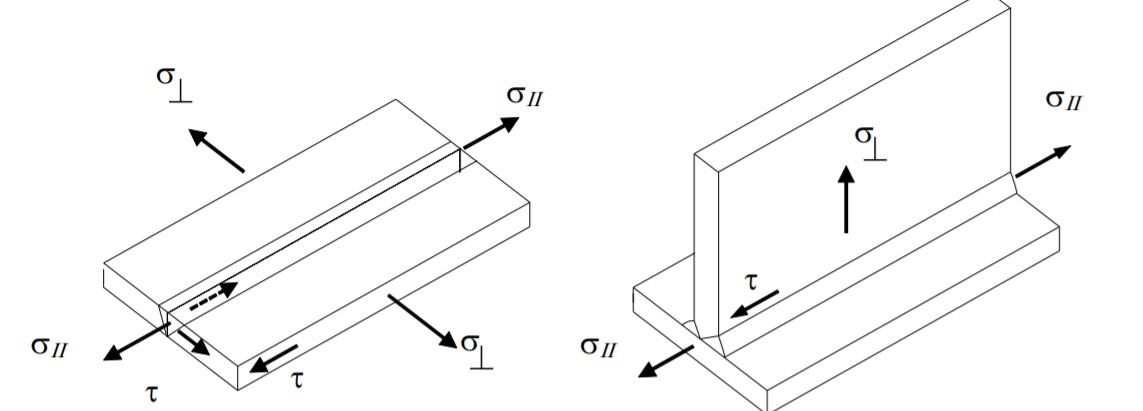
\includegraphics[width=8cm]{fpj-stresses} 
		\caption{stress components on a  full penetration joint.} \label{fig:fpjstresses}
	\end{SCfigure}

	To verify such stress state usually the Von Mises failure criterion is used assuming a plane stress state giving
	\begin{equation}
		\seq = \sqrt{\sigma_\parallel^2 + \sigma_\perp^2 - \sigma_\parallel \sigma_\perp + 3\tau^2} \leq \sigma_{W,all} = \nu \sall
	\end{equation}
	where $\sall$ is the allowable stress of the filler material (table \ref{tab:weldsall}) and $\nu$ is the \textbf{weakening coefficient} that might be $\nu=1$ for $1^{st}$ class joints (high quality) and $\nu=0.85$ for $2^{nd}$ class joints (medium quality).
	
	\begin{table}[bht]
		\centering
		\rule{0.9\linewidth}{1pt}
		\caption{allowable stress $\sall$ by the welds for different materials and section thicknesses.}
		\label{tab:weldsall}		
		\begin{tabular}{c | c c }
			\multirow{2}{*}{steel} & \multicolumn{2}{c}{$\sall [MPa]$} \\
			& thickness $< 40mm$ & thickness $> 40mm$ \\ \hline
			\texttt{S235} & 160 & 140  \\
			\texttt{S275} & 190 & 170  \\
			\texttt{S355} & 240 & 210  \\
			
		\end{tabular}
		\rule{0.9\linewidth}{1pt}
	\end{table}
	
\subsection{Fillet joints}
	Fillet joints do not restore the structural continuity of the joined parts; particular attention must be paid to the definition of the resisting cross-section area and the stress states.	After experimental result's analysis, the stress components were calculated on the throat area but to simplify the stress analysis we consider the throat as overturned on a convenient side of the joint (figure \ref{fig:fjstresses}). With such choice the verification criteria becomes
	\begin{equation}
	\begin{aligned}
		\sqrt{\sigma_\perp^2 + \tau_\perp^2 + \tau_\parallel^2} & \leq \nu_1 \sall \\ |\sigma_\perp| + |\tau_\perp| & \leq \nu_2 \sall
	\end{aligned}
	\end{equation}
	where $\nu_1 < \nu_2$ are two (different) weakening coefficient that takes into account ductility and weldability.
	
	\begin{SCfigure}[1][bht]
		\centering 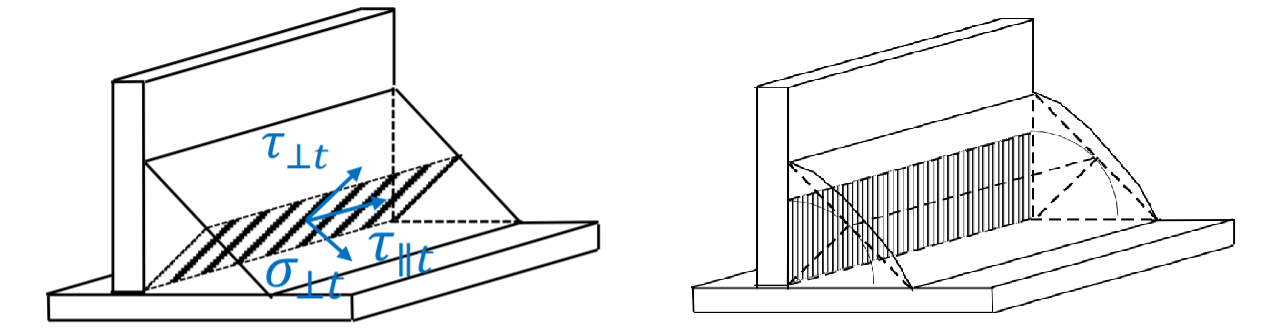
\includegraphics[width=9cm]{fj-stress}
		\caption{stress components referred to the throat area (left) and the related over-turned area (right).} \label{fig:fjstresses}
	\end{SCfigure}
	
\subsection*{Stress components}
	To determine stress components we can use typical stress distribution analysis considering the throat area (for full penetration joints) or the \textit{easier} overturned area (fillet joints).